\documentclass{article}
\usepackage{amsmath}
\usepackage{amssymb}
\usepackage{graphicx}
\usepackage{ctex}
\usepackage{subfigure}
\begin{document}
\title{第二次作业}
\maketitle
\begin{minipage}[b]{0.5\linewidth}
学号:190320517\\
姓名:葛旭\\
班级:自动化五班\\
\end{minipage}
\hfill
\begin{minipage}[b]{0.5\linewidth}
\includegraphics[width=0.45\textwidth]{gexu.eps}\\
\end{minipage}
1.C\\
2.C\\
3.D\\
4.C\\
5.B\\
6.C\\
7.\[\begin{gathered}
(1){u_1} = \sqrt {\frac{G}{\rho }} (S - wave) = 3500m/s \Rightarrow G = \rho u_1^2 = 3.43 \times {10^{10}} \hfill \\
{u_2} = \sqrt {\frac{E}{\rho }} (P - wave) = 5500m/s \Rightarrow E = \rho u_2^2 = 8.47 \times {10^{10}} \hfill \\
(2){\text{suppose the distance is x}} \hfill \\
\frac{x}{{3500}} - \frac{x}{{5500}} = 12 \Rightarrow x = 1.155 \times {10^5}m \hfill \\ 
\end{gathered} \]
9.\[\begin{gathered}
(1)A = 0.2m,u = \frac{\lambda }{T} = \frac{\omega }{k} = 2.5m/s,T = \frac{{2\pi }}{\omega } = 0.8s \hfill \\
\upsilon  = \frac{1}{T} = 1.25{s^{ - 1}},\lambda  = uT = 2m \hfill \\
(2)v = \frac{{\partial y}}{{\partial t}} =  - 0.5\pi \sin (2.5\pi t - \pi x) \hfill \\
{\text{so the largest velocity is 0}}{\text{.5}}\pi {\kern 1pt} {\kern 1pt} {\kern 1pt} {\text{m/s}}{\text{.}} \hfill \\
(3)t = 1s,y = 0.2\cos (2.5\pi  - \pi x) = 0.2\sin (\pi x) \hfill \\
t = 2s,y = 0.2\cos (5\pi  - \pi x) =  - 0.2\cos (\pi x) \hfill \\
x = 1m,y = 0.2\cos (2.5\pi t - \pi ) =  - 0.2\cos (2.5\pi t) \hfill \\ 
\end{gathered} \]
波形图是t为一个常数时所有质点的位置图象,第三个是某一个质点随时间t的位置变化。
\begin{figure}[htbp]
	\centering
	
	\subfigure[$y=0.2\sin (\pi x)$]{
		\begin{minipage}[t]{0.5\linewidth}
			\centering
			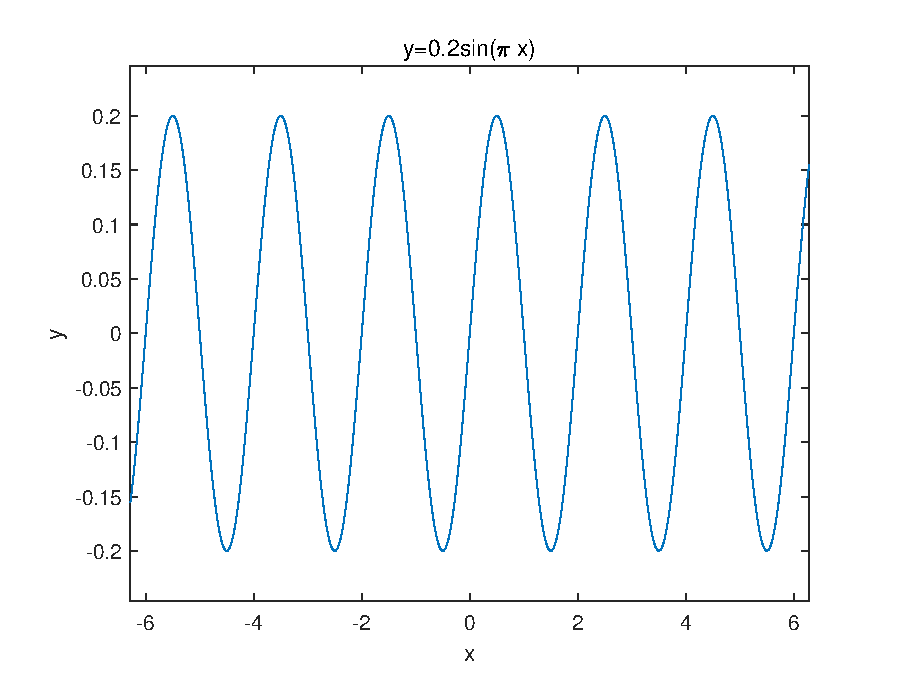
\includegraphics[width=2in]{10-9-1.eps}
			%\caption{fig1}
		\end{minipage}%
	}%
	\subfigure[$y=-0.2\cos (\pi x)$]{
		\begin{minipage}[t]{0.5\linewidth}
			\centering
			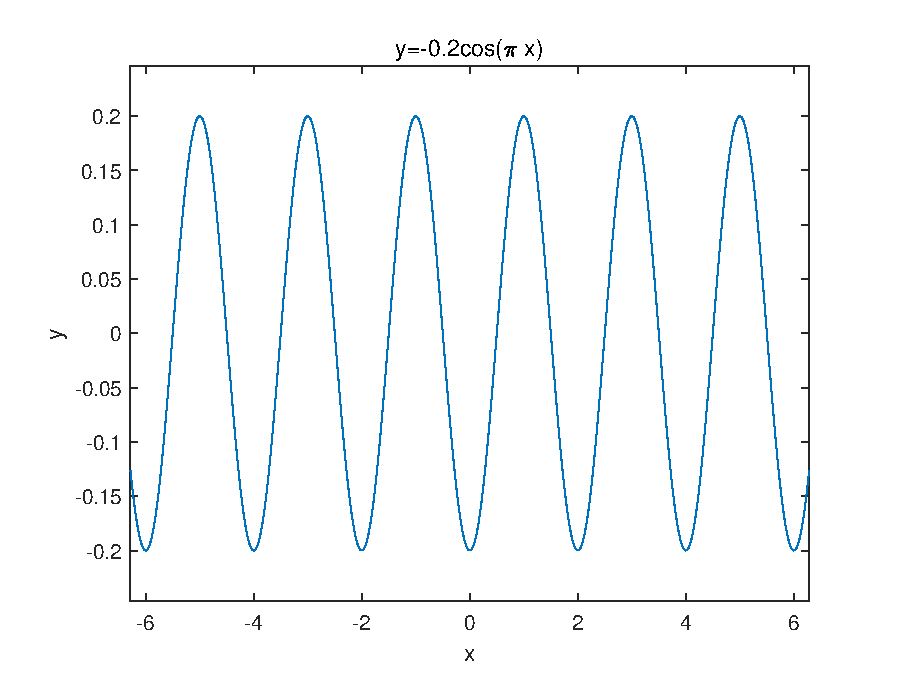
\includegraphics[width=2in]{10-9-2.eps}
			%\caption{fig2}
		\end{minipage}%
	}%
	\\
	%这个回车键很重要 \quad也可以
	\subfigure[$y=-0.2\cos (2.5\pi t)$]{
		\begin{minipage}[t]{0.9\linewidth}
			\centering
			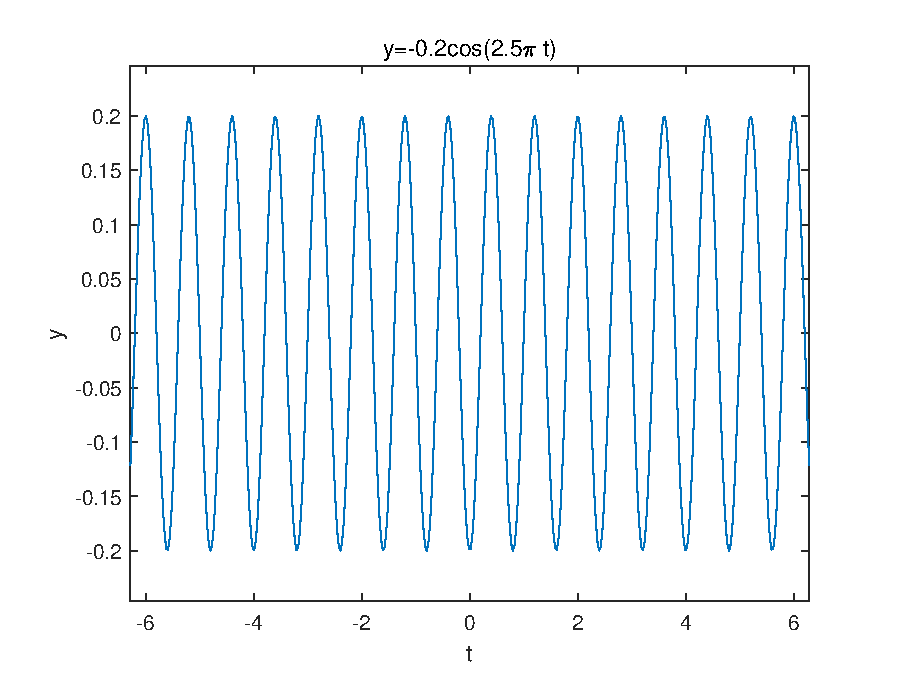
\includegraphics[width=2.5in]{10-9-3.eps}
			%\caption{fig2}
		\end{minipage}
	}%
	
	\centering
	\caption{10-9}
\end{figure}\\
10.\[\begin{gathered}
(1)T = \frac{{2\pi }}{\omega } = \frac{1}{{120}}s,\lambda  = uT = \frac{1}{4}m \hfill \\
(2)k = \frac{{2\pi }}{\lambda } = 8\pi ,y = 4 \times {10^{ - 3}}\cos (240\pi t - 8\pi x) \hfill \\ 
\end{gathered} \]
11.\[\begin{gathered}
(1)T = \frac{{2\pi }}{\omega } = \frac{1}{2}s,\lambda  = uT = 10m,k = \frac{{2\pi }}{\lambda } = \frac{\pi }{5} \hfill \\
\Rightarrow y = 3 \times {10^{ - 2}}\cos (4\pi t + \frac{\pi }{5}x + \pi ) =  - 3 \times {10^{ - 2}}\cos (4\pi t + \frac{\pi }{5}x) \hfill \\
(2){\text{B is later than A,so}} \hfill \\
\Rightarrow \Delta \varphi  = kx = \pi ,y = 3 \times {10^{ - 2}}\cos (4\pi t + \frac{\pi }{5}x + \pi  - \pi ) = 3 \times {10^{ - 2}}\cos (4\pi t + \frac{\pi }{5}x) \hfill \\ 
\end{gathered} \]
12.\[\begin{gathered}
(1)T = \frac{{2\pi }}{\omega } = \frac{1}{5}s,\upsilon  = \frac{1}{T} = 5{s^{ - 1}},k = 2 = \frac{{2\pi }}{\lambda },\lambda  = \pi ,u = \frac{\lambda }{T} = 5\pi m/s \hfill \\
(2)y = 0.05\sin (10\pi t) \hfill \\ 
\end{gathered} \]
x=0时的方程的意义即为x=0处的质点随时间的振动图像。
\begin{figure}[!h]
	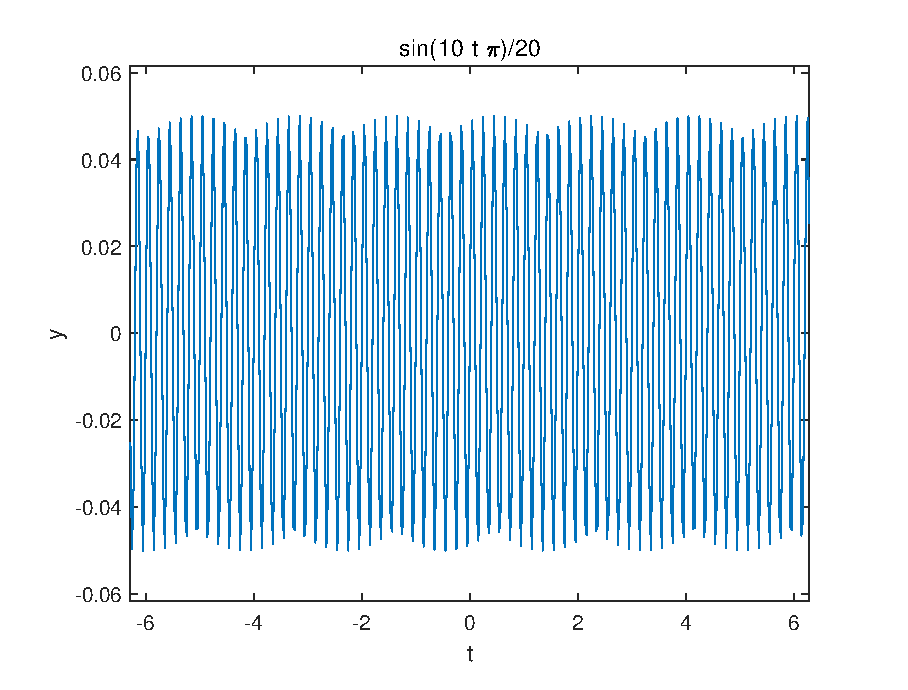
\includegraphics[width=1.05\textwidth]{10-12.eps}
\end{figure}\\
13.\[\begin{gathered}
(1)T = 0.02s,u = 100m/s,\varphi  =  - \frac{\pi }{2},\lambda  = uT = 2m \hfill \\
\omega  = \frac{{2\pi }}{T} = 100\pi rad/s,k = \frac{{2\pi }}{\lambda } = \pi  \hfill \\
{\text{the wave equation is :}}y = A\cos (100\pi t - \pi x + \varphi ) \hfill \\
x = 15m:y = A\cos (100\pi t - 15\pi  - \frac{\pi }{2}) = A\cos (100\pi t - 15.5\pi ),{\text{the initial phase is }} - 15.5\pi . \hfill \\
x = 5m:y = A\cos (100\pi t - 5\pi  - \frac{\pi }{2}) = A\cos (100\pi t - 5.5\pi ),{\text{the initial phase is }} - 5.5\pi . \hfill \\
(2)\Delta \varphi  = \frac{{2\pi }}{\lambda }\Delta r = \pi  \hfill \\ 
\end{gathered} \]
14.\[\begin{gathered}
(a){\text{wave equation:}}y = A\cos (\omega t - kx + \varphi ),P:y = A\cos (\omega t - kb + \varphi ) \hfill \\
(b){\text{wave equation:}}y = A\cos (\omega t + kx + \varphi ),P:y = A\cos (\omega t - kb + \varphi ) \hfill \\
(c){\text{wave equation:}}y = A\cos (\omega t - k(x - l) + \varphi ),P:y = A\cos (\omega t - kb + \varphi ) \hfill \\ 
\end{gathered} \]
15.\[\begin{gathered}
(1)A = 0.1m,{\varphi _0} = \frac{\pi }{3},\lambda  = 20m,\nu  = 250Hz,u = \lambda \nu  = 5000m/s,k = \frac{{2\pi }}{\lambda } = \frac{\pi }{{10}} \hfill \\
\Rightarrow y = 0.1\cos (500\pi t + \frac{\pi }{3} + \frac{\pi }{{10}}x) \hfill \\
({\text{2}})x = 7.5m,y = 0.1\cos (500\pi t + \frac{{13\pi }}{{12}}),\frac{{dy}}{{dt}} =  - 50\pi \sin (500\pi t + \frac{{13\pi }}{{12}}) \hfill \\
t = 0,\frac{{dy}}{{dt}} =  - 50\pi \sin (\frac{{13\pi }}{{12}}) = 40.6m/s \hfill \\ 
\end{gathered} \]
16.\[\begin{gathered}
(1)A = 0.04m,\lambda  = 0.4m,u = 0.08m/s,T = \frac{\lambda }{u} = 5s \hfill \\
k = \frac{{2\pi }}{\lambda } = 5\pi ,\omega  = \frac{{2\pi }}{T} = \frac{{2\pi }}{5},{\varphi _0} = \frac{\pi }{2} \hfill \\
y = 0.04\cos (\frac{{2\pi }}{5}t - 5\pi x - \frac{\pi }{2}) = 0.04\sin (\frac{{2\pi }}{5}t - 5\pi x) \hfill \\
(2)x = 0.2m,y = 0.04\sin (\frac{{2\pi }}{5}t - \pi ) =  - 0.04\sin (\frac{{2\pi }}{5}t) \hfill \\ 
\end{gathered} \]
17.\[\begin{gathered}
\lambda  = 12m,{\text{suppose the wave equation is }}y = A\cos (\omega t + kx + \varphi ) \hfill \\
x = 1m,\varphi  =  - \frac{\pi }{2},y = A\cos (\omega t + \frac{{2\pi }}{\lambda } + \varphi ) = A\cos (\omega t + \frac{\pi }{6} - \frac{\pi }{2}) \hfill \\
\omega t = \frac{\pi }{3} + \frac{\pi }{2} = \frac{{5\pi }}{6},t = 5s,\omega  = \frac{\pi }{6}rad/s \hfill \\
\Rightarrow {\text{so the wave equation is }}y = 0.4\cos (\frac{\pi }{6}t + \frac{\pi }{6}x - \frac{\pi }{2}) \hfill \\ 
\end{gathered} \]
20.\[\begin{gathered}
{I_1}4\pi r_1^2 = P \Rightarrow {I_1} = \frac{P}{{4\pi r_1^2}} = 1.27 \times {10^{ - 2}}W/{m^2} \hfill \\
{I_2}4\pi r_2^2 = P \Rightarrow {I_2} = \frac{P}{{4\pi r_2^2}} = 3.18 \times {10^{ - 3}}W/{m^2} \hfill \\ 
\end{gathered} \]
21.\[\begin{gathered}
(1)I = \frac{1}{2}\rho {A^2}{\omega ^2}u = 2{\pi ^2}\rho {A^2}{\nu ^2}u = 1.58 \times {10^5}W/{m^2} \hfill \\
(2)w = ISt = 3.79 \times {10^3}J \hfill \\ 
\end{gathered} \]
23.\[\begin{gathered}
(1)\Delta \varphi  = \frac{{2\pi }}{\lambda }\frac{{3\lambda }}{2} = 3\pi  \hfill \\
(2)A = \sqrt {A_1^2 + A_2^2 + 2{A_1}{A_2}\cos \varphi }  = |{A_1} - {A_2}| \hfill \\ 
\end{gathered} \]
24.\[\begin{gathered}
{\text{suppose the midpoint between A and B is O}} \hfill \\
{\text{(1)when the point is on the left of A:}} \hfill \\
\Delta \varphi  = {\varphi _B} - {\varphi _A} - \frac{{2\pi }}{\lambda }({r_B} - {r_A}) =  - 14\pi ,{\text{there is no still point}} \hfill \\
{\text{(2)when the point is on the right of B:}} \hfill \\
\Delta \varphi  = {\varphi _B} - {\varphi _A} - \frac{{2\pi }}{\lambda }({r_B} - {r_A}) = 16\pi ,{\text{there is no still point}} \hfill \\
{\text{(3)when the point is between A and B:}} \hfill \\
{\text{suppose the coordinate of the point is }}x,{r_A} = 15 - x,{r_B} = 15 + x \hfill \\
\Delta \varphi  = {\varphi _B} - {\varphi _A} - \frac{{2\pi }}{\lambda }({r_B} - {r_A}) = \pi (x + 1) = (2k + 1)\pi  \Rightarrow x = 2k \hfill \\
x =  - 14m, - 12m, \cdots ,12m,14m \hfill \\ 
\end{gathered} \]
27.\[\begin{gathered}
{\text{the standard standing wave equation is :}} \hfill \\
y = 2A\cos (kx)\cos (\omega t) \hfill \\
(1)k = \frac{{2\pi }}{\lambda } = 1.6\pi ,\lambda  = 1.25m,\omega  = 550\pi ,A = 0.015,\nu  = 275Hz \hfill \\
u = \lambda \nu  = 343.8m/s \hfill \\
(2)\Delta x = \frac{\lambda }{2} = 0.625m \hfill \\
(3)\frac{{dy}}{{dt}} = 0.03 \times 550\pi  \times \cos (1.6\pi x)( - \sin (550\pi t)),t = 3 \times {10^{ - 3}}s,x = 0.625 \hfill \\
\frac{{dy}}{{dt}} =  - 46.2m/s \hfill \\ 
\end{gathered} \]
28.\[\begin{gathered}
{y_1} + {y_2} = 0.12\cos (\frac{1}{2}\pi  \times 0.02x)\cos (\frac{1}{2}\pi  \times 8t) = 0.12\cos (0.01\pi x)\cos (4\pi t) \hfill \\
0.12\cos (0.01\pi x) = 0.06 \Rightarrow x = 200k \pm \frac{{100}}{3} m \hfill \\ 
\end{gathered} \]
29.\[\begin{gathered}
(1)close:\nu  = \frac{u}{{u - v}}{\nu _0} = 865.6Hz \hfill \\
far:\nu  = \frac{u}{{u + v}}{\nu _0} = 743.7Hz \hfill \\
(2)\nu  = \frac{{u - {v_s}}}{{u - v}} = 826.2Hz \hfill \\ 
\end{gathered} \]
30.\[\begin{gathered}
(1)\nu ' = \frac{{u + {v_2}}}{{u - {v_1}}} = 1022Hz \hfill \\
(2)\nu '' = \frac{{u + {v_1}}}{{u - {v_2}}} = 1045Hz \hfill \\ 
\end{gathered} \]
\end{document}